% ------------------------------------------------------------------------
%                                 Portada
% ------------------------------------------------------------------------

\thispagestyle{empty}

\begin{center}

DISCRIMINACIÓN DEL RUIDO DE FONDO EN MUOGRAFÍA USANDO TÉCNICAS DE APRENDIZAJE AUTOMATIZADO \vspace{6cm}

ALEJANDRO RAMIREZ MUÑOZ\\DAVID VILLABONA ARDILA
\vspace{6cm}

UNIVERSIDAD INDUSTRIAL DE SANTANDER\\
FACULTAD DE INGENIERÍAS FÍSICOMECÁNICAS\\
ESCUELA DE INGENIERÍA DE SISTEMAS E INFORMÁTICA\\
BUCARAMANGA\\
2021\\

\end{center}

% ------------------------------------------------------------------------
%                              Contraportada
% ------------------------------------------------------------------------

\newpage
\thispagestyle{empty}

\begin{center}

DISCRIMINACIÓN DEL RUIDO DE FONDO EN MUOGRAFÍA USANDO TÉCNICAS DE MACHINE LEARNING \vspace{1cm}

ALEJANDRO RAMIREZ MUÑOZ\\DAVID VILLABONA ARDILA\\
\vspace{1cm}

Trabajo de Grado para optar al título de\\
Ingeniero de Sistemas.\\\vspace{1cm}

Director\\
JESÚS PEÑA RODRÍGUEZ\\

\vspace{1cm}

Codirector\\
LUIS ALBERTO NÚÑEZ DE VILLAVICENCIO MARTÍNEZ\\
\\FABIO MARTÍNEZ CARILLO\\
\vspace{1cm}


UNIVERSIDAD INDUSTRIAL DE SANTANDER\\
FACULTAD DE INGENIERÍAS FÍSICOMECÁNICAS\\
ESCUELA DE INGENIERÍA DE SISTEMAS E INFORMÁTICA\\
BUCARAMANGA\\
2021\\

\end{center}
% ------------------------------------------------------------------------
%                             Nota de proyecto
% ------------------------------------------------------------------------

%\newpage
%\pagenumbering{arabic} \setcounter{page}{3}

%\begin{figure}
%\begin{center}
%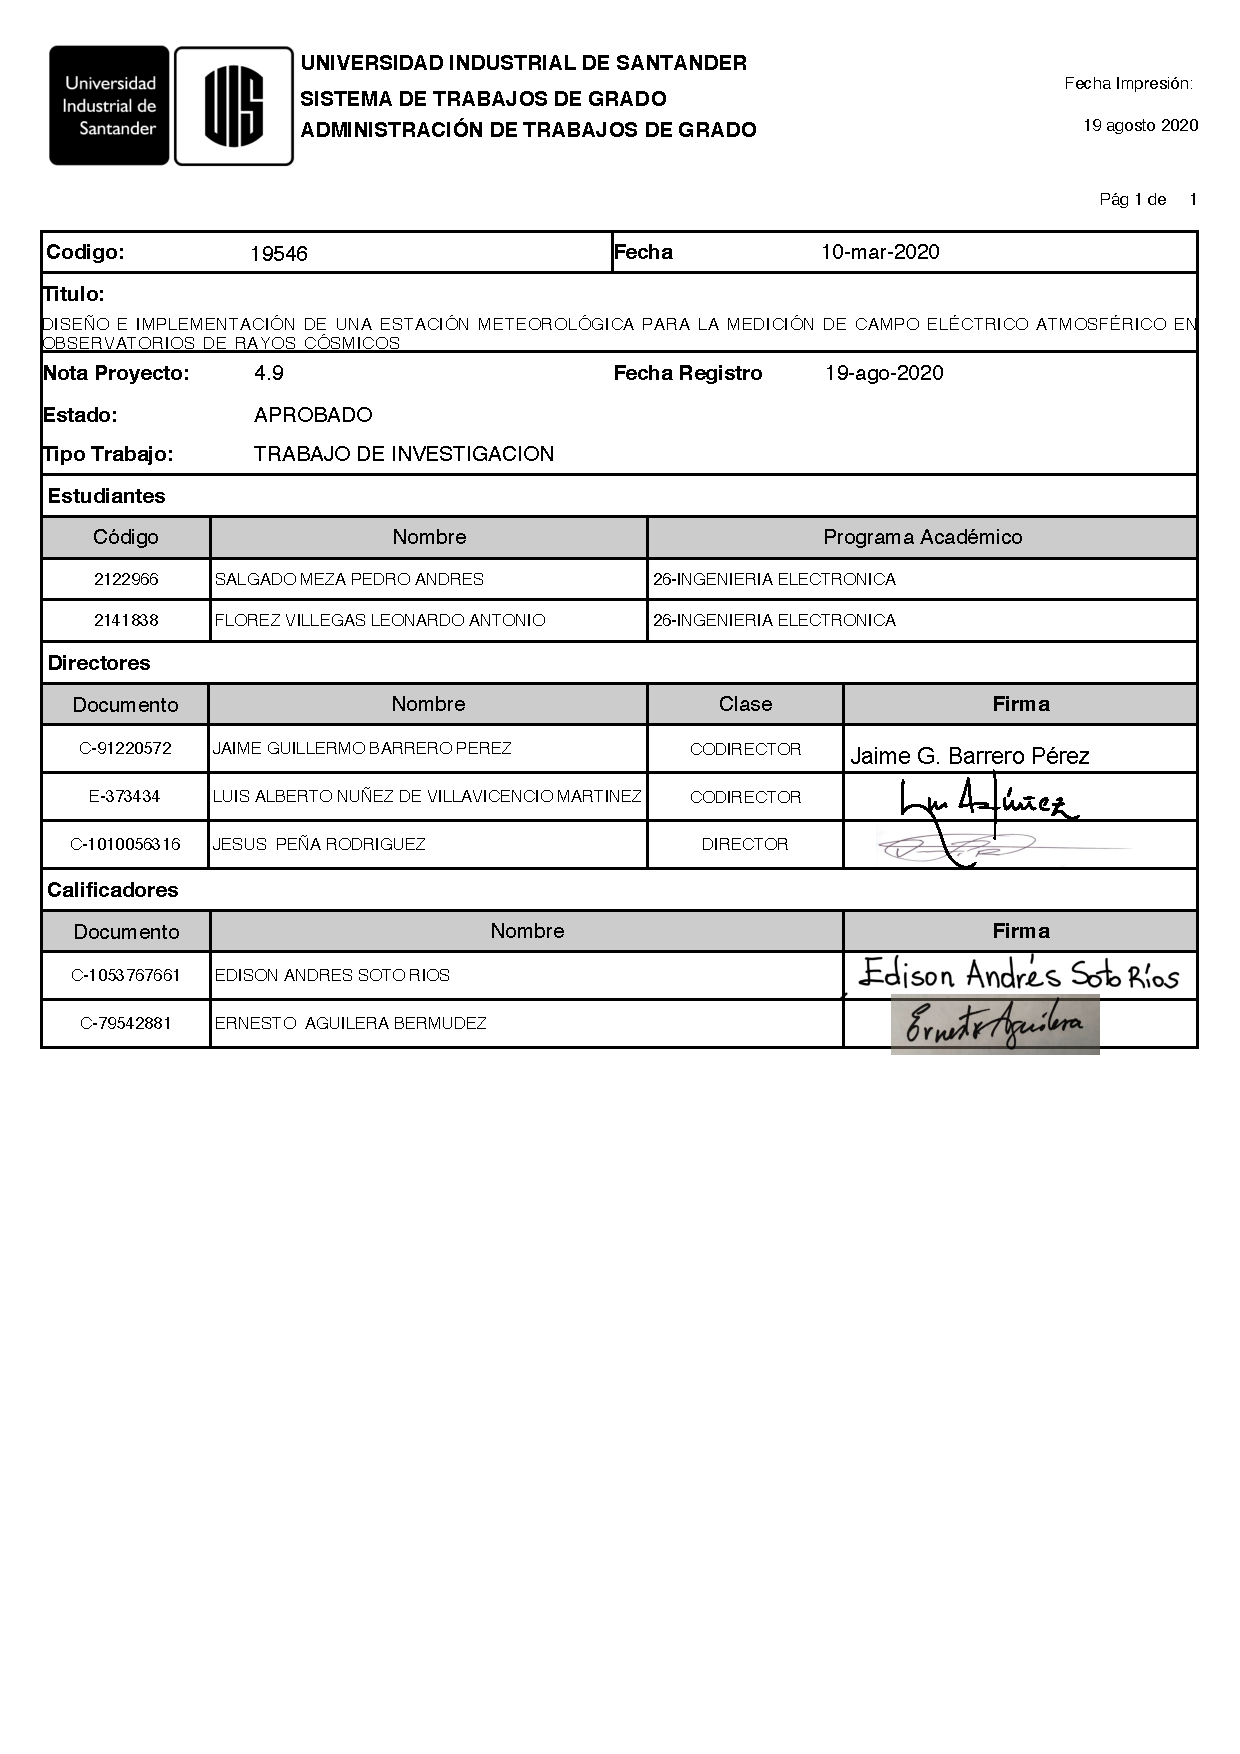
\includegraphics[width=1\textwidth]{acta.pdf}
%\end{center}
%\end{figure}

% ------------------------------------------------------------------------
%                             Autorización
% ------------------------------------------------------------------------

%\newpage

%\begin{figure}
%\begin{center}
%\includegraphics[width=1\textwidth]{autorizacion_g%rado.pdf}
%\end{center}
%\end{figure} 
% ----------------------